\documentclass[11pt,a4paper]{report}
\usepackage[spanish,es-nodecimaldot]{babel}	% Utilizar español
\usepackage[utf8]{inputenc}					% Caracteres UTF-8
\usepackage{graphicx}						% Imagenes
\usepackage[hidelinks]{hyperref}			% Poner enlaces sin marcarlos en rojo
\usepackage{fancyhdr}						% Modificar encabezados y pies de pagina
\usepackage{float}							% Insertar figuras
\usepackage[textwidth=390pt]{geometry}		% Anchura de la pagina
\usepackage[nottoc]{tocbibind}				% Referencias (no incluir num pagina indice en Indice)
\usepackage{enumitem}						% Permitir enumerate con distintos simbolos
\usepackage[T1]{fontenc}					% Usar textsc en sections
\usepackage{amsmath}						% Símbolos matemáticos

% Comando para poner el nombre de la asignatura
\newcommand{\asignatura}{Simulación de Sistemas}
\newcommand{\autor}{José María Sánchez Guerrero}
\newcommand{\titulo}{Práctica 2}
\newcommand{\subtitulo}{Modelos de Monte Carlo. Generadores de datos}

% Configuracion de encabezados y pies de pagina
\pagestyle{fancy}
\lhead{\autor{}}
\rhead{\asignatura{}}
\lfoot{Grado en Ingeniería Informática}
\cfoot{}
\rfoot{\thepage}
\renewcommand{\headrulewidth}{0.4pt}		% Linea cabeza de pagina
\renewcommand{\footrulewidth}{0.4pt}		% Linea pie de pagina

\begin{document}
\pagenumbering{gobble}

% Pagina de titulo
\begin{titlepage}

\begin{minipage}{\textwidth}

\centering


\includegraphics[scale=0.5]{img/ugr.png}\\

\textsc{\Large \asignatura{}\\[0.2cm]}
\textsc{GRADO EN INGENIERÍA INFORMÁTICA}\\[1cm]

\noindent\rule[-1ex]{\textwidth}{1pt}\\[1.5ex]
\textsc{{\Huge \titulo\\[0.5ex]}}
\textsc{{\Large \subtitulo\\}}
\noindent\rule[-1ex]{\textwidth}{2pt}\\[3.5ex]

\end{minipage}

\vspace{0.5cm}

\begin{minipage}{\textwidth}

\centering

\textbf{Autor}\\ {\autor{}}\\[2.5ex]
\textbf{Rama}\\ {Computación y Sistemas Inteligentes}\\[2.5ex]
\vspace{0.3cm}


\includegraphics[scale=0.3]{img/etsiit.jpeg}

\vspace{0.7cm}
\textsc{Escuela Técnica Superior de Ingenierías Informática y de Telecomunicación}\\
\vspace{1cm}
\textsc{Curso 2019-2020}
\end{minipage}
\end{titlepage}

\pagenumbering{arabic}
\tableofcontents
\thispagestyle{empty}				% No usar estilo en la pagina de indice

\newpage

\setlength{\parskip}{1em}

\chapter{Mi segundo modelo de simulación de MonteCarlo}

Un establecimiento se abastece diariamente de un cierto producto, y necesita decidir cuántas unidades \textbf{s} de ese producto
pedir cada día Se desea encontrar el valor de $s$ donde se maximice la ganancia esperada. Obtenemos una ganancia de \textbf{x}
euros por unidad vendida, y una pérdida de \textbf{y} euros si no se ha vendido al final del dia. También contaremos con un valor
de demanda, el cual serán los productos solicitados cada día y seguirán una distribución de probabilidad \textbf{P} con el cual
jugaremos para ver los distintos resultados que nos ofrecerán.


\section{Experimentación inicial}

Empezaremos por un modelo de MonteCarlo inicial, en el cual representaremos todas las variables anteriores en el código para calcular
la ganancia, y también dispondremos de varias distribuciones para calcular la demanda de productos solicitados. La ganancia viene
determinada por lo siguiente:

\begin{equation}
	g(s,x,y,d)=\left\{\begin{matrix}
	x*s\hspace{27mm}si\hspace{2mm}d\geq s\\ 
	x*d-(s-d)*y\hspace{6mm}si\hspace{2mm}d\geq s
	\end{matrix}\right.
\end{equation}

Y tendremos estas tres tipos de distribuciones que podremos seleccionar en el código la que queramos. Hay que tener en cuenta que la
simulación será para 100 valores de $s$, por lo que esto influirá también en las distribuciones:

\begin{itemize}
	\item $P(D=d)$ se distribuye uniformemente entre 0 y 99
	\item $P(D=d)$ es proporcional a $100-d$, $\forall d=0,1,2,...,99$
	\item $P(D=d)$ tiene una distribución "triangular" que crece con $d/2500$ entre 0 y 50; y decrece con $(100-d)/2500$ entre 50 y 99.
\end{itemize}

Por último, como vamos a ejecutar un modelo varias \textbf{veces}, tendremos que obtener la media para cada $s$ y también la desviación
típica con la fórmula
\begin{equation}
	desviaciont=\sqrt{\frac{sum2-veces*gananciaesperada*gananciaesperada}{veces-1}}
\end{equation}

El código de este ejercicio está en el archivo $generadores.c$, proporcionado junto a la memoria. Vamos a ejecutarlo con distintos parámetros
para ver cómo afectan al modelo. La ejecución la vamos a dividir en tres: una para $x=10, y=1$; otra para $x=10, y=5$; y la última para
$x=10, y=10$. Los valores de las tablas serán tanto la ganancia como la desviación típica para los distintos valores de $veces$ y
contrastaremos los resultados.

Estos han sido los resultados para la distribución \textbf{uniforme}:

\begin{table}[H]
	\parbox{.45\linewidth}{
	\centering
	\begin{tabular}{c|ccc}
	\textbf{Veces} & \textbf{s} & \textbf{Ganancia} & \textbf{Desviación} \\ \hline
	\textbf{100}   & 86         & 495.68            & 316.09			  \\ \hline
	\textbf{1000}  & 91         & 472.38            & 308.29			  \\ \hline
	\textbf{5000}  & 90         & 457.66            & 310.85 			  \\ \hline
	\textbf{10000} & 91         & 454.09            & 311.94			  \\ \hline
	\textbf{100000}& 87         & 450.85            & 304.69			  \\
	\end{tabular}
	\caption{$x=10$, $y=1$}
	}
	\hfill
	\parbox{.45\linewidth}{
	\centering
	\begin{tabular}{c|ccc}
	\textbf{Veces} & \textbf{s} & \textbf{Ganancia} & \textbf{Desviación} \\ \hline
	\textbf{100}   & 77         & 390.80            & 388.73			  \\ \hline
	\textbf{1000}  & 70         & 347.14            & 348.71			  \\ \hline
	\textbf{5000}  & 67         & 335.88            & 332.22 			  \\ \hline
	\textbf{10000} & 65         & 333.65            & 323.97			  \\ \hline
	\textbf{100000}& 66         & 330.05            & 331.99			  \\
	\end{tabular}
	\caption{$x=10$, $y=5$}
	}
\end{table}
\begin{table}[H]
	\centering
	\begin{tabular}{c|ccc}
	\textbf{Veces} & \textbf{s} & \textbf{Ganancia} & \textbf{Desviación} \\ \hline
	\textbf{100}   & 50         & 290.60            & 314.91			  \\ \hline
	\textbf{1000}  & 55         & 268.84            & 356.97			  \\ \hline
	\textbf{5000}  & 48         & 254.50            & 306.41 			  \\ \hline
	\textbf{10000} & 53         & 249.94            & 345.77			  \\ \hline
	\textbf{100000}& 51         & 247.03            & 333.85			  \\
	\end{tabular}
	\caption{$x=10$, $y=10$}
\end{table}

A simple vista se puede observa como los resultados se van ajustando cada vez mejor a medida que aumentamos el número de repeticiones. Es lo
lógico, ya que cuantas más veces se pruebe el modelo, más real será la media entre todos los valores (teniendo en cuenta que se utilizan valores
aleatorios y siempre vamos a tener un pequeño error).

Todo lo contrario con los resultados que ofrecen las cantidades de repeticiones bajas. Es difícil fiarnos de un resultado así, y menos sabiendo
que el modelo depende bastante de la aleatoriedad, y que cualquier valor fuera de lo normal hace que cambie todo de una forma más acentuada que
en uno con más repeticiones.

No obstante, hay que tener en cuenta que cuantas más repeticiones le pongamos, más tardará en ejecutarse. En estos ejemplos no tenemos mucho
problema en eso, ya que son bastante rápidos pese a ejecutarlo con $veces=100000$.

Si nos fijamos ahora en como cambian los valores entre tablas, es decir, entre unos valores de $y$ y otros, vemos como para un valor más bajo
las ganancias son más altas que con un valor alto. Esto tiene sentido, porque la $y$ representa cuanto aumentan las pérdidas si tenemos muchos
productos sin vender.

En el caso de la $y=1$ las ganancias y los productos adquiridos ($s$) son muy altos, ya que apenas perdemos si no vendemos una unidad; en cambio,
con la $y=10$ la ganancia baja y los productos adquiridos también, ya que no sale rentable comprarlos y después tener que desecharlos.

Vamos a probar ahora con otra distribución. Estos han sido los resultados para la distribución \textbf{proporcional}:
\begin{table}[H]
	\parbox{.45\linewidth}{
	\centering
	\begin{tabular}{c|ccc}
	\textbf{Veces} & \textbf{s} & \textbf{Ganancia} & \textbf{Desviación} \\ \hline
	\textbf{100}   & 78         & 322.40            & 285.75			  \\ \hline
	\textbf{1000}  & 69         & 297.04            & 243.19			  \\ \hline
	\textbf{5000}  & 71         & 289.95            & 244.48 			  \\ \hline
	\textbf{10000} & 72         & 287.13            & 227.74			  \\ \hline
	\textbf{100000}& 67         & 283.75            & 235.86			  \\
	\end{tabular}
	\caption{$x=10$, $y=1$}
	}
	\hfill
	\parbox{.45\linewidth}{
	\centering
	\begin{tabular}{c|ccc}
	\textbf{Veces} & \textbf{s} & \textbf{Ganancia} & \textbf{Desviación} \\ \hline
	\textbf{100}   & 57         & 233.40            & 293.49			  \\ \hline
	\textbf{1000}  & 44         & 202.47            & 229.51			  \\ \hline
	\textbf{5000}  & 39         & 193.12            & 203.07 			  \\ \hline
	\textbf{10000} & 42         & 193.25            & 221.17			  \\ \hline
	\textbf{100000}& 44         & 188.60            & 231.17			  \\
	\end{tabular}
	\caption{$x=10$, $y=5$}
	}
\end{table}
\begin{table}[H]
	\centering
	\begin{tabular}{c|ccc}
	\textbf{Veces} & \textbf{s} & \textbf{Ganancia} & \textbf{Desviación} \\ \hline
	\textbf{100}   & 30         & 167.40            & 210.69			  \\ \hline
	\textbf{1000}  & 30         & 146.60            & 201.91			  \\ \hline
	\textbf{5000}  & 27         & 136.17            & 179.10 			  \\ \hline
	\textbf{10000} & 27         & 135.01            & 178.65			  \\ \hline
	\textbf{100000}& 28         & 133.66            & 189.31			  \\
	\end{tabular}
	\caption{$x=10$, $y=10$}
\end{table}

Vemos que el resto de valores son más bajos que en las tablas anteriores. En este caso no tenemos analíticamente el valor de $s$ para contrastar el
resultado, pero por la forma decreciente de la distribución utilizada podemos decir que estos valores tienen sentido. Una distribución decreciente
quiere decir que las demandas pequeñas tienen más posibilidades de salir que las grandes, es decir, que la gente comprará menos ese producto y no 
tendremos que adquirir tantos.

Por otra parte, cuantas más repeticiones ponemos, al igual que antes, más exactos salen nuestros resultados. Lo mismo sucede con los valores de $y$
respecto a $x$, y es que para un valor más bajo las ganancias son más altas que con un valor alto.

Por último vamos a analizar los resultados para la distribución \textbf{triangular}:
\begin{table}[H]
	\parbox{.45\linewidth}{
	\centering
	\begin{tabular}{c|ccc}
	\textbf{Veces} & \textbf{s} & \textbf{Ganancia} & \textbf{Desviación} \\ \hline
	\textbf{100}   & 83         & 493.40            & 217.66			  \\ \hline
	\textbf{1000}  & 77         & 476.39            & 212.23			  \\ \hline
	\textbf{5000}  & 76         & 466.11            & 205.99 			  \\ \hline
	\textbf{10000} & 76         & 466.78            & 206.22			  \\ \hline
	\textbf{100000}& 79         & 464.94            & 212.76			  \\
	\end{tabular}
	\caption{$x=10$, $y=1$}
	}
	\hfill
	\parbox{.45\linewidth}{
	\centering
	\begin{tabular}{c|ccc}
	\textbf{Veces} & \textbf{s} & \textbf{Ganancia} & \textbf{Desviación} \\ \hline
	\textbf{100}   & 74         & 432.50            & 282.03			  \\ \hline
	\textbf{1000}  & 62         & 408.09            & 225.36			  \\ \hline
	\textbf{5000}  & 59         & 389.14            & 218.78 			  \\ \hline
	\textbf{10000} & 58         & 388.80            & 215.32			  \\ \hline
	\textbf{100000}& 59         & 386.79            & 221.56 			  \\
	\end{tabular}
	\caption{$x=10$, $y=5$}
	}
\end{table}
\begin{table}[H]
	\centering
	\begin{tabular}{c|ccc}
	\textbf{Veces} & \textbf{s} & \textbf{Ganancia} & \textbf{Desviación} \\ \hline
	\textbf{100}   & 51         & 367.00            & 225.96			  \\ \hline
	\textbf{1000}  & 44         & 335.26            & 187.24			  \\ \hline
	\textbf{5000}  & 53         & 336.00            & 251.46 			  \\ \hline
	\textbf{10000} & 48         & 337.11            & 217.58			  \\ \hline
	\textbf{100000}& 49         & 333.64            & 228.09			  \\
	\end{tabular}
	\caption{$x=10$, $y=10$}
\end{table}

Al igual que ha pasado con las otras dos distribuciones, nos vamos a quedar con los resultados que nos han ofrecido las repeticiones más altas, ya que
son los más fiables. Más de lo mismo con la relación $x-y$, aunque en este caso vemos como esta vez los valores no están tan lejos los unos de otros.

Analizando los resultados que nos ofrece la $s$, vemos como los valores rondan el $n/2$ (en nuestro caso 50), porque la distribución triangular hace
que los valores más probables estén por ahí. Esto también ha afectado a los valores de la ganancia, que en esta tabla hemos visto que son más altos que
en los anteriores. Esto nos es muy útil, ya que si tuviesemos datos reales o una distribución real de la gente que compra los productos, podríamos ajustar
un modelo MonteCarlo a los números aleatorios de esta distribución. El objetivo de esto sería obviamente ajustar las variables para obtener la ganancia
más alta posible.


\section{Modificaciones del modelo}

\subsection{Cantidad fija de devolución}

En este apartado vamos a modificar el modelo construido anteriormente, de tal forma que el establecimiento pueda devolver las unidades no vendidas. De 
esta forma hay que pagar una cantidad fija de $z$ euros de gastos de devolución de las unidades no vendidas, en vez de tener una pérdida de $y$ euros por
unidad. Esta cantidad no varía, a menos que la $z=0$.

La función de ganancia ahora sería:
\begin{equation}
	g(s,x,y,d)=\left\{\begin{matrix}
	x*s\hspace{12mm}si\hspace{2mm}d\geq s\\ 
	x*d-z\hspace{5mm}si\hspace{2mm}d\geq s
	\end{matrix}\right.
\end{equation}

Estará implementada en el código $generadoresModificados.c$ y las pruebas que vamos a realizar van a ser con el número de repeticiones más alto, que ya
hemos visto que es el más fiable (100000 veces) y con los tres tipos de distribuciones. El resultado ha sido el siguiente:

\begin{table}[H]
	\centering
	\begin{tabular}{c|cccc}
	\textbf{\hspace{5mm}z\hspace{5mm}}   & \textbf{Distribución} & \textbf{\hspace{5mm}s\hspace{5mm}} & \textbf{Ganancia} & \textbf{Desviación} \\ \hline
	\textbf{5}   & uniforme 			 & 95         & 490.45            & 297.18 			  \\
	\textbf{5}   & proporcional			 & 91         & 326.41            & 236.09			  \\
	\textbf{5}   & triangular 			 & 95         & 495.37            & 203.63			  \\ \hline
	\textbf{400} & uniforme 			 & 59         & 178.91            & 367.37 			  \\
	\textbf{400} & proporcional			 & 20         & 18.58             & 246.17			  \\
	\textbf{400} & triangular 		     & 44         & 233.82            & 273.39			  \\ \hline
	\textbf{200} & uniforme 			 & 79         & 318.07            & 317.13 			  \\
	\textbf{200} & proporcional		     & 61         & 142.47            & 255.30			  \\
	\textbf{200} & triangular 		     & 55         & 323.75            & 214.21			  \\
	\end{tabular}
	\caption{Resultados para todas las distribuciones con $x=10$ y $veces=100000$}
\end{table}

Lo hemos ejecutado con un valor de $y=5$ ya que no era ni tan bajo que apenas supusiese pérdidas, ni tan alto que no diese demasiadas. Puede ser que
no sea el valor más adecuado, pero para lo que queremos mostrar, nos servirá.

En la ejecución vemos cómo las distribuciones se adecuan bastante bien a lo que comentamos en el punto anterior sobre ellas. Por otro lado, vamos a
analizar los resultados que nos ofrece cada $z$, que es realmente lo interesante en este apartado. Vemos que los valores bajos, como puede ser el 5,
hace que la cantidad de productos pedidos sea muy alta. Esto se debe a que la pérdidas por cada producto no vendido van a ser muy pocas.

Por otro lado, con los valores altos, como puede ser el 400, los valores ya empiezan a ser mucho más bajos, tanto en la cantidad de productos como en
las ganancias que obtenemos. Esto es porque, pese a que ajustemos las ventas al máximo, con que nos sobren muy pocos productos ya estaremos pagando un
precio muy alto (razón por la cual las ganancias también disminuyen).

Estos valores son poco realista, porque ni una empresa te va a cobrar una excesiva cantidad de dinero por delvolver el producto, ni te va a cobrar tan
poco que no les salga rentable a ellos. Por eso, ahora vamos a probar con un valor que se puede ajustar mejor, como puede ser el 200. Podemos ver que los
valores de $s$ no están mal ajustados, dependiendo del tipo de distribución, y que las ganancias están bastante bien (claramente son más altas las que nos
ofrecen los $z$ pequeños, pero no sería un valor realista).


\subsection{Cantidad relativa de devolución}

Por último, vamos a 'fusionar' los dos últimos casos en uno. Si el valor $z$ es relativamente grande, no interesará pagar esa cantidad
de dinero cuando queden pocas unidades sin vender. Por otro lado, cuando el número de unidades no vendidas sea pequeño, es preferible asumir
la pérdidas de $y$ que tener que pagar los gastos de devolución.

La función de la ganancia se nos quedaría de la siguiente forma:
\begin{equation}
	g(s,x,y,d)=\left\{\begin{matrix}
	x*s\hspace{37mm}si\hspace{2mm}d\geq s\\ 
	x*d-min\{z,(s-d)*y\}\hspace{4mm}si\hspace{2mm}d\geq s
	\end{matrix}\right.
\end{equation}

También estará implementada en $generadoresModificados.c$, y para ejecutarla, tendremos que cambiar el parámetro $modificacion=2$. El resto
de valores, se mantendrán exactamente iguales que en las ejecuciones anterior. Los resultados han sido los siguientes:

\begin{table}[H]
	\centering
	\begin{tabular}{c|cccc}
	\textbf{\hspace{5mm}z\hspace{5mm}}   & \textbf{Distribución} & \textbf{\hspace{5mm}s\hspace{5mm}} & \textbf{Ganancia} & \textbf{Desviación} \\ \hline
	\textbf{100} & uniforme 			 & 92         & 411.21            & 309.86 			  \\
	\textbf{100} & proporcional			 & 72         & 238.44            & 247.52			  \\
	\textbf{100} & triangular 			 & 74         & 415.98            & 217.21			  \\ \hline
	\textbf{150} & uniforme 			 & 86         & 380.06            & 327.23 			  \\
	\textbf{150} & proporcional			 & 56         & 206.16            & 249.46			  \\
	\textbf{150} & triangular 		     & 61         & 396.93            & 211.83			  \\ \hline
	\textbf{200} & uniforme 			 & 81         & 356.57            & 317.13 			  \\
	\textbf{200} & proporcional		     & 43         & 189.64            & 225.30			  \\
	\textbf{200} & triangular 		     & 60         & 390.21            & 219.63			  \\
	\end{tabular}
	\caption{Resultados para todas las distribuciones con $x=10$, $y=5$ y $veces=100000$}
\end{table}

En esta ejecución podemos ver como para un valor intermedio de $y$ cómo cambian los resultados. Estos se modifican siguiendo las mismas reglas comentadas
anteriormente, pero en este caso vemos aumentadas las ganancias debido a que elegimos cual nos conviene más, si pagar una cantidad fija o variable.

\begin{table}[H]
	\centering
	\begin{tabular}{c|cccc}
	\textbf{\hspace{5mm}y\hspace{5mm}}   & \textbf{Distribución} & \textbf{\hspace{5mm}s\hspace{5mm}} & \textbf{Ganancia} & \textbf{Desviación} \\ \hline
	\textbf{3} & uniforme 			 	 & 79         & 381.69            & 334.20 			  \\
	\textbf{3} & proporcional			 & 54         & 225.98            & 240.16			  \\
	\textbf{3} & triangular 			 & 64         & 419.09            & 210.75			  \\ \hline
	\textbf{7} & uniforme 			 	 & 83         & 344.55            & 337.87 			  \\
	\textbf{7} & proporcional		     & 51         & 172.44            & 258.79			  \\
	\textbf{7} & triangular 		     & 59         & 373.18            & 225.49			  \\ \hline
	\textbf{10} & uniforme 				 & 81         & 336.49            & 335.62 			  \\
	\textbf{10} & proporcional			 & 53         & 162.06            & 260.66			  \\
	\textbf{10} & triangular 		     & 57         & 358.21            & 222.97			  \\
	\end{tabular}
	\caption{Resultados para todas las distribuciones con $x=10$, $z=200$ y $veces=100000$}
\end{table}

En este caso hemos elegido un $z=200$ para ver como cambian las tablas en función de la $y$. Como podemos ver, los modelos de MonteCarlo son bastante flexibles
y gracias a ellos podemos ajustar las variables a las que más nos convengan o las que más se adecuen a nuestra situación. En estos casos, quizás el gerente
de la tienda no pueda controlar ni las pérdidas que le da cada producto o los precios de devolución ($y$ y $z$ respectivamente), pero sí puede controlar la
cantidad de productos que adquiera y adecuarla a las distintas situaciones que se pueden dar, y que en definitiva, más ganancia le den.




\chapter{Generadores de datos}

En esta otra parte de la práctica vamos a intentar mejorar los generadores de datos, ya que es una parte fundamental a la hora de ejecutar nuestros modelos.
Un generador lo más aleatorio posible, que se adecue a las distintas situaciones que nos propongan los modelos y que además sea eficiente, sería el ideal, y 
es lo que vamos a buscar en este capítulo. El código se encontrará en el archivo 'generadoresMejorados.c', donde habrá distintas funciones alternativas que
muestren los cambios realizados.

\section{Mejorando los generadores}

\subsection{Generadores ordenados}

Vamos a intentar mejorar la eficiencia de los generadores de datos empleados en el capítulo anterior. La primera mejora que vamos a aplicar va a ser la ordenación
de las tablas de forma decreciente según la probabilidad. Como los generadores $a$ y $b$ (uniforme y proporcional respectivamente), vamos a centrarnos en el
generador $c$ o triangular. La ejecución ha sido probada con 1000000 de repeticiones, para que se vea mejor cómo afecta y los resultados han sido los siguientes:
\begin{figure}[H]
\centering
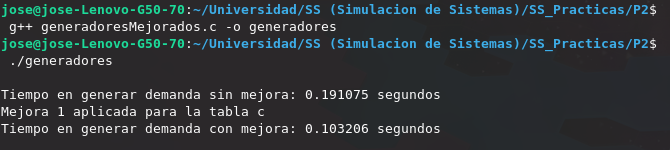
\includegraphics[scale=0.7]{img/mejora1.png}
\caption{Ejecución con el tiempo sin y con mejora del generador c}
\end{figure}

Vemos que se reduce el tiempo a casi la mitad. Esto se debe a que, al estar ordenado de más probabilidad a menos, los valores que más van a salir serán encontrados
antes en la tabla. Pese a esto, sigue siendo una tabla y la búsqueda de ellos va a ser lineal, es decir, va a recorrer los valores uno a uno hasta llegar al correcto.


\subsection{Implementación con búsqueda binaria}

En este apartado modificaremos todos los generadores. Como hemos dicho anteriormente, la búsqueda lineal era un problema, asi que en este caso vamos a implementar
una búsqueda binaria que solucione el problema. En el código, se cambiará la función $genera\_demanda$ por $genera\_demanda\_binaria$. Este es el resultado que nos
ofrece:
\begin{figure}[H]
\centering
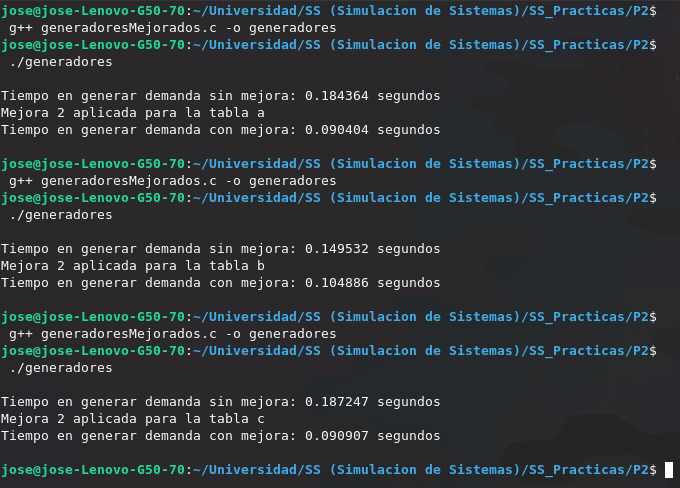
\includegraphics[scale=0.6]{img/mejora2.png}
\caption{Ejecución con los tiempos sin y con mejora de búsqueda}
\end{figure}

Podemos ver que en el generador c los resultados son todavía mejores que antes, mientras que en los otros dos generadores también ha dado unos buenos resultados.
Esto se debe a que hemos pasado de hacer una búsqueda de orden lineal a una búsqueda de orden logarítmico. La mejora se ha notado sobre todo en el primer generador,
y en el último, donde ha bajado el tiempo casi un 50\%; mientras que en el generador $b$ ha sido un poco menos.


\subsection{Mejora de eficiencia constante en el generador a}

Por último, vamos a probar a mejorar la eficiencia del generador uniforme haciendo que su tiempo de ejecución sea constante. Este generador lo que hace es generar
un número aleatorio y recorrer la tabla hasta encontrar un valor mayor que este, y devolver el índice donde estaba situado. Nos podemos ahorrar este proceso si,
tras generar el número aleatorio entre 0 y 1, lo multiplicamos por 100 y nos quedamos con la parte entera.

Los resultados obtenido tras implementarlo han sido:
\begin{figure}[H]
\centering
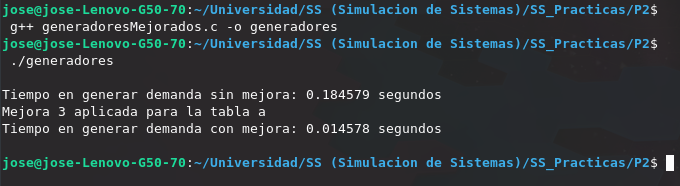
\includegraphics[scale=0.7]{img/mejora3.png}
\caption{Ejecución con los tiempos sin y con mejora del generador a}
\end{figure}

Vemos que la mejora ha sido muy grande, mucho mejor que las anteriores. Lo bueno de este método es que, por muchos elementos que tengamos, la eficiencia va a ser
la misma, porque estamos ante una 'búsqueda' de orden constante. En contra de este método, decir que funciona porque el generador original en uniforme, pero a
la hora de hacerlo para los generadores nos resultará imposible encontrar algo similar.


\newpage

\section{Generadores congruenciales}

En esta sección vamos a analizar los generadores básicos y ver el peligro que conlleva no implementarlos de forma correcta. El ejercicio nos pide implementar
dos generadores congruenciales de la siguiente forma:
\begin{equation}
x_{n+1} = (2061x_n + 4321) \mod m
\end{equation}

Y el otro muy similar:
\begin{equation}
x_{n+1} = (2060x_n + 4321) \mod m
\end{equation}

El código donde está implementados se llama $generadoresCongruencias.c$ y para cambiar entre uno y otro sólo tendremos que cambiar la variable $a=2060$ o
$a=2061$. El ejercicio también nos pide que se calcule el número de periodos obtenidos con distintos tipos de aritméticas: entera, real 'artesanal', real
'artesanal' corregida y real usando $fmod$. Para cambiar de aritmética sólo tendremos que cambiar la variable $aritmetica$ en el código.

También tendremos que seleccionar un valor de $m=10^4$ y un valor inicial $x_0=14$ en mi caso. El resultado de las ejecuciones ha sido el siguiente:

\begin{table}[H]
	\centering
	\begin{tabular}{c|c|c}
	\textbf{Aritmética}	& \textbf{Periodo gen 1} & \textbf{Periodo gen 2} \\ \hline
	entera   			& 10000         		 & 4 					  \\ \hline
	real artesanal		& 152         			 & 8					  \\ \hline
	artesanal corregida & 10000        			 & 4				  	  \\ \hline
	real con $fmod$ 	& 10000        			 & 4				  	  \\
	\end{tabular}
	\caption{$x=10$, $y=10$}
\end{table}

Podemos ver cómo claramente el generador 2 (cuya $a=2060$) no es un buen generador de números aleatorios, ya que empezará a repetir valores muy temprano, por
otro lado, el generador 1 es un generador correcto, ya que llaga a los $10^4$ periodos sin repetir ni un número. Esto se debe a que $a$ y $m$ no tienen
divisores en común, mientras que con el generador 2 no sucede lo mismo.

Si nos fijamos en la aritmética real artesanal, vemos como termina muy pronto, en comparación al resto de aritméticas del generador 1. La razón por la que
sucede esto es que no se redondea correctamente el valor obtenido, es decir, si yo obtengo el 0.99, esta aritmética lo tomará como 0, estando claramente este
valor más cerca del 1.

Podemos decir que el resto de aritméticas estan bien hechas, ya que ninguna de ellas comenten estos errores y consiguen alcanzar el periodo máximo.



\end{document}

